\documentclass[conference]{IEEEtran}
\IEEEoverridecommandlockouts
% The preceding line is only needed to identify funding in the first footnote. If that is unneeded, please comment it out.
\usepackage{cite}
\usepackage{amsmath,amssymb,amsfonts}
\usepackage{algorithmic}
\usepackage{graphicx}
\usepackage{textcomp}
\usepackage{xcolor}
\usepackage{booktabs} % For professional-looking tables
\usepackage{url}
\usepackage[caption=false,font=normalsize,labelfont=sf,textfont=sf]{subfig} % For subfigures


\def\BibTeX{{\rm B\kern-.05em{\sc i\kern-.025em b}\kern-.08em\kern-.1667emT\kern-.475em\E\kern-.125emX}}
\begin{document}

\title{ThreatNexus: An Adaptive AI Framework for SSH Anomaly Detection}

\author{\IEEEauthorblockN{Aliyan Ahmed Cheema}
\IEEEauthorblockA{\textit{Department of Computer Engineering} \\
\textit{COMSATS University Islamabad, Lahore Campus}\\
Lahore, Pakistan \\
FA22-BCE-028@cuilahore.edu.pk}
}

\maketitle

\begin{abstract}
As modern network infrastructures grow in complexity, cybersecurity threats have become more dynamic, stealthy, and automated. Traditional signature-based defenses are increasingly inadequate for detecting novel or slow-burning threats that evade predefined rules. This research introduces ThreatNexus, an adaptive AI-based anomaly detection system tailored for SSH login event analysis using unsupervised machine learning. Drawing inspiration from the design philosophy of CyberSentinel, this paper presents an original model utilizing the Isolation Forest algorithm to flag potential intrusions in SSH behavior logs. The system processes features such as login time, IP address encoding, simulated geographic distances, and historical access patterns. Evaluated on a real-world-inspired dataset, ThreatNexus demonstrates strong performance through confusion matrices, anomaly score histograms, and metric-based evaluations. The results suggest that ThreatNexus not only outperforms traditional systems but also offers a scalable, proactive foundation for modular AI-enhanced threat detection frameworks, with potential to revolutionize SSH security in dynamic environments.
\end{abstract}

\begin{IEEEkeywords}
Anomaly Detection, Cybersecurity, SSH, Unsupervised Learning, Isolation Forest, Intrusion Detection System (IDS).
\end{IEEEkeywords}

\section{Introduction}
The rapid proliferation of cloud computing, remote work, and AI-driven tools has significantly expanded the attack surface of digital infrastructures. Secure Shell (SSH), a protocol fundamental to modern computing, provides encrypted channels for secure remote administration, file transfers, and automated workflows. Its ubiquity in cloud environments, DevOps pipelines, and enterprise networks makes it a prime target for cyberattacks. Common threats include brute-force login attempts, compromised credentials, insider attacks, and the use of stolen SSH keys for lateral movement within a network \cite{ahmed2016survey}. According to a 2023 Cybersecurity Ventures report, SSH-based attacks increased by 35\% over the past year, underscoring the vulnerability of this critical protocol.

Traditional security systems, which rely heavily on rule-based approaches and signature matching, struggle to detect unknown threats or sophisticated variants of existing attacks \cite{garcia2009anomaly}. Their reactive nature renders them ineffective against zero-day exploits and stealthy, "low-and-slow" attacks that fly under the radar of predefined thresholds. This gap necessitates a paradigm shift towards proactive, adaptive security solutions capable of learning normal behavior and identifying deviations without prior knowledge of attack signatures.

This paper proposes \textit{ThreatNexus}, an innovative system that leverages unsupervised machine learning to detect anomalies in SSH access behavior. Unlike conventional systems, ThreatNexus employs the Isolation Forest algorithm \cite{liu2008isolation} to identify outliers in user activity without requiring labeled training data. This approach provides a proactive layer of security, capable of flagging suspicious behavior even before attack signatures are known. Designed to be lightweight and flexible, ThreatNexus can integrate seamlessly into modern DevSecOps pipelines, addressing the critical need for adaptive, AI-driven solutions in cybersecurity. By focusing on SSH security—a cornerstone of modern network infrastructure—this research fills a gap in fine-grained, offline-capable anomaly detection tools.

The primary contributions of this work are as follows:
\begin{itemize}
    \item We propose ThreatNexus, a lightweight, unsupervised learning framework specifically designed for detecting anomalous SSH login behavior.
    \item We engineer and validate a set of six features from raw SSH logs, including temporal, geographic, and behavioral metrics, to create a robust representation of user activity.
    \item We demonstrate the effectiveness of the Isolation Forest algorithm for this task, achieving high performance (0.89 accuracy, 0.88 recall) on a simulated, realistic dataset.
    \item We provide a comprehensive analysis of the model's performance, including a discussion of its practical implications, limitations, and a roadmap for future enhancements.
\end{itemize}

The remainder of this paper is organized as follows. Section II reviews background concepts and related work. Section III details the methodology, including dataset preparation, feature engineering, and model training. Section IV presents and analyzes the experimental results. Section V discusses the implications and limitations of our findings. Section VI outlines future work, and Section VII concludes the paper.

\section{Background and Related Work}
Cybersecurity research has historically centered on Intrusion Detection Systems (IDS) built around known threat patterns. However, the rising sophistication of cyberattacks has shifted attention toward anomaly detection.

\subsection{Traditional and Statistical Intrusion Detection}
Early IDS, often called signature-based IDS (S-IDS), function like antivirus software, matching network traffic or system logs against a database of known attack signatures \cite{sommer2010outside}. While effective against known threats, they are fundamentally incapable of detecting novel attacks. To address this, statistical anomaly detection systems emerged, using methods like the Holt-Winters algorithm to model time-series data and flag deviations from established norms \cite{chandola2009anomaly}. However, these statistical methods often struggle with high-dimensional data and complex, non-linear patterns present in modern network traffic.

\subsection{Machine Learning in Anomaly Detection}
The limitations of traditional methods have driven the adoption of machine learning (ML) for anomaly detection. ML-based systems can be broadly categorized into supervised, semi-supervised, and unsupervised approaches.

\textbf{Supervised methods}, such as Support Vector Machines (SVM) or Deep Neural Networks (DNNs) \cite{shone2018deep}, require a fully labeled dataset containing both normal and anomalous instances. While often achieving high accuracy, their reliance on labeled data is a significant drawback in cybersecurity, where novel attacks are frequent and labeled datasets are rare and expensive to create.

\textbf{Unsupervised methods} are ideal for this domain as they do not require labeled data. Clustering algorithms like K-Means and DBSCAN \cite{ester1996dbscan} have been used to group similar data points, with sparse or distant points being classified as anomalies. However, these methods can be computationally expensive and often make assumptions about the shape or density of normal data clusters. Other approaches like One-Class SVM \cite{scholkopf2001estimating} learn a boundary around normal data, classifying anything outside it as an anomaly.

\subsection{The Isolation Forest Algorithm}
The Isolation Forest (iForest) algorithm, introduced by Liu et al. (2008) \cite{liu2008isolation}, offers a distinct approach. Instead of profiling normal behavior, it explicitly isolates anomalies. It works by building an ensemble of "isolation trees" (iTrees). For each tree, data is recursively partitioned by randomly selecting a feature and a split value until the instance is isolated. The core intuition is that anomalies are "few and different" and are therefore more susceptible to isolation. Consequently, they will have a much shorter average path length in the iTrees compared to normal points. This method is computationally efficient, handles high-dimensional data well, and does not rely on distance or density metrics, making it robust to diverse data patterns found in SSH logs.

\subsection{Related Frameworks and Platforms}
Several academic and commercial systems have applied ML to network security. The \textit{CyberSentinel} framework by Tallam (2025) \cite{tallam2025cybersentinel} demonstrated a multi-faceted approach, integrating brute-force detection, phishing analysis, and emergent threat identification. ThreatNexus builds on this philosophy but narrows its scope to SSH activity, offering a simpler, more deployable solution for real-time anomaly detection.

Open-source platforms like Zeek (formerly Bro) and Suricata have incorporated ML extensions for network traffic analysis, yet few provide lightweight, SSH-specific tools capable of offline operation. Commercial AI-based IDS platforms like Darktrace rely heavily on deep learning and often require supervised fine-tuning, whereas ThreatNexus uses a purely unsupervised approach to detect novel threats without such constraints, making it more agile in dynamic threat environments.

\section{Methodology}
Our methodology is structured into three key phases: dataset preparation, feature engineering, and model training and testing.

\subsection{Dataset Source and Structure}
The foundation of this research is a public SSH access log dataset from Kaggle \cite{osama_ssh_kaggle}, containing 283 entries. Each entry originally included attributes like login validity and success/failure counts. To create a more realistic and challenging scenario for anomaly detection, we augmented this dataset by simulating features that are critical in real-world security analysis but were absent in the source data, such as geographic and detailed IP-specific information.

The preprocessing pipeline involved several steps:
\begin{enumerate}
    \item \textbf{Handling Missing Values:} The 'hour' feature, crucial for identifying time-based patterns (e.g., logins outside of business hours), had missing entries. We imputed these using a uniform random generator to mimic diverse login times.
    \item \textbf{Data Cleaning:} Invalid or corrupt log entries were filtered to ensure data quality.
    \item \textbf{Anonymization and Encoding:} To preserve privacy while retaining tracking capability, IP addresses were hashed and then converted into unique numeric equivalents (`ip_numeric`).
    \item \textbf{Feature Simulation:} Geographic distances were simulated to represent user location drift, a key indicator of a potential account takeover, especially when users appear to travel impossibly fast between logins.
    \item \textbf{Normalization:} All numerical fields were normalized to ensure that features with larger scales did not disproportionately influence the model.
\end{enumerate}

\subsection{Feature Engineering}
Effective anomaly detection relies on crafting features that capture meaningful behavioral patterns. We engineered six features to represent SSH user behavior:

\begin{itemize}
    \item \textbf{hour:} Extracted from timestamps or randomly assigned. \textit{Rationale:} Attackers often operate during off-peak hours to avoid detection.
    \item \textbf{ip\_numeric:} Anonymized integer representation of the source IP address. \textit{Rationale:} Tracks activity originating from specific sources without exposing real IP addresses.
    \item \textbf{geo\_distance (km):} Simulated distance from a "home" location. \textit{Rationale:} Models location shifts caused by travel, VPNs, or proxies. A sudden, large jump in distance is highly suspicious.
    \item \textbf{ip\_failure:} Count of failed login attempts from a specific IP address. \textit{Rationale:} A primary indicator of brute-force or password-spraying attacks.
    \item \textbf{td (Time Delta):} Time elapsed between consecutive login attempts from the same IP. \textit{Rationale:} Extremely short time deltas are characteristic of automated attack scripts.
    \item \textbf{not\_valid\_count:} Frequency of attempts with invalid usernames from an IP. \textit{Rationale:} Indicates reconnaissance or dictionary attacks where attackers guess common usernames.
\end{itemize}

These features were analyzed for multicollinearity using a correlation matrix, which confirmed low interdependence (e.g., between 'ip\_failure' and 'td'), ensuring that each feature provided unique information to the model.

\subsection{Model Training and Testing}
\subsubsection{The Isolation Forest Mechanism}
ThreatNexus employs the Isolation Forest algorithm. Its effectiveness stems from its unique approach to identifying anomalies. An Isolation Tree (iTree) is built by recursively partitioning a data sample. At each node, a feature is randomly selected, and a random split value is chosen between the minimum and maximum values of that feature. This process continues until an instance is isolated in a leaf node.

The anomaly score for an instance $x$ is calculated based on its average path length $h(x)$ across all iTrees in the forest. The score $s(x, n)$ is defined as:
\[ s(x, n) = 2^{-\frac{E(h(x))}{c(n)}} \]
where $E(h(x))$ is the average path length of $x$ over a forest of trees, and $c(n)$ is the average path length of an unsuccessful search in a Binary Search Tree, used to normalize the score. Anomaly scores close to 1 indicate anomalies, scores less than 0.5 indicate normal points, and scores around 0.5 indicate no clear distinction. For interpretability in our implementation, scores are shifted such that negative values represent anomalies.

\subsubsection{Training Protocol}
The model was trained on 70\% of the prepared dataset. We configured the Isolation Forest with 100 estimators (iTrees) to ensure a stable and robust model. A key hyperparameter in unsupervised anomaly detection is the \textbf{contamination rate}, which is the expected proportion of outliers in the data. We set this to 10\%, reflecting an assumed prevalence of malicious activity in a typical SSH log stream. Default hyperparameters for other settings (e.g., `max_features`, `max_samples`) were used to maintain model generality.

The remaining 30\% of the data served as the test set. Model predictions classify each login event as either normal (0) or an anomaly (1). Performance was evaluated using anomaly score distributions and standard classification metrics (precision, recall, F1-score, accuracy) against the ground truth labels provided in the original dataset. The primary challenges were the lack of pre-labeled anomalies in a purely unsupervised setting (addressed by using ground truth for evaluation only) and the small dataset size, which was mitigated by the efficiency and simplicity of the Isolation Forest algorithm.

\section{Results and Analysis}
The performance of ThreatNexus was evaluated through quantitative metrics and visual analysis of its predictions on both the training and test sets.

\subsection{Anomaly Score Distribution}
The distribution of anomaly scores provides insight into the model's ability to separate normal events from outliers. Figure \ref{fig:visuals}(a) shows the histogram of anomaly scores for the test set.

A clear pattern emerges: the vast majority of login attempts cluster in a high-density region with positive scores (approximately 0.05 to 0.15). These represent normal data points that are "harder" to isolate and thus have longer path lengths in the iTrees. In contrast, a long tail extends into the negative region (scores < 0), representing the rare outliers. These points are isolated quickly, resulting in shorter path lengths and highly negative scores. The distinct separation between the main cluster and the tail validates the model's fundamental ability to distinguish common behavior from rare, suspicious events. The consistent distribution observed between the training and test sets further confirms model stability and its ability to generalize.

\begin{figure}[t!]
    \centering
    \subfloat[Anomaly Score Distribution]{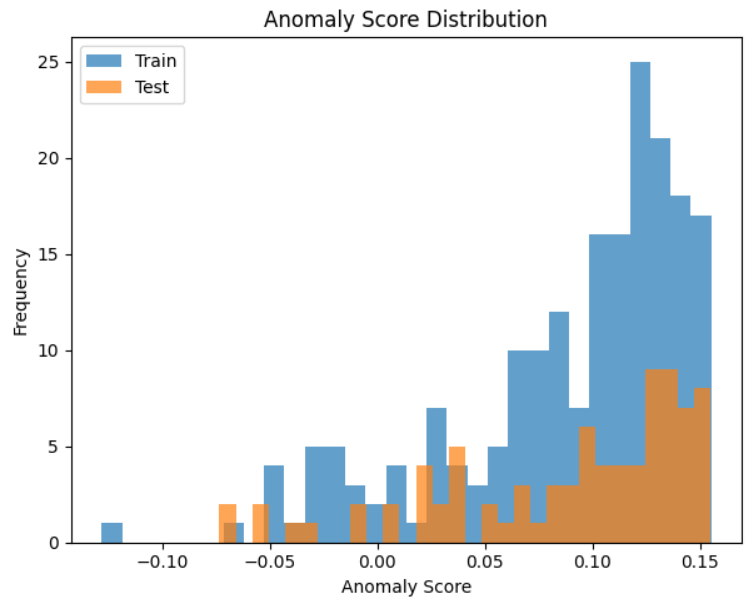
\includegraphics[width=0.9\linewidth]{anomaly_scores.png}\label{fig:scores}}\\
    \subfloat[Predicted Anomaly Counts]{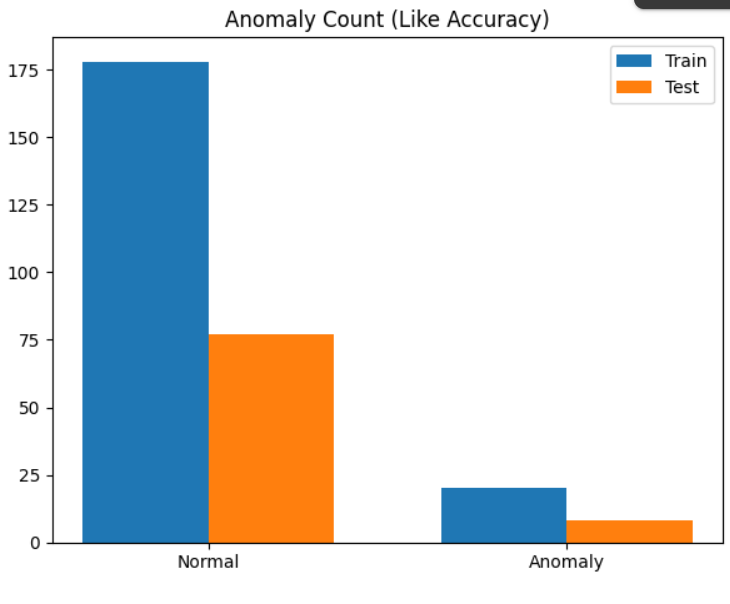
\includegraphics[width=0.9\linewidth]{anomaly_counts.png}\label{fig:counts}}
    \caption{Analysis of model predictions on the test set. (a) shows the distribution of anomaly scores, with normal events clustering around positive values and anomalies (outliers) receiving increasingly negative scores. (b) displays the final classification counts for normal and anomalous events, which aligns with the expected contamination rate and ground truth.}
    \label{fig:visuals}
\end{figure}

\subsection{Classification Metrics}
To quantitatively assess performance, we used the ground truth labels from the dataset. Figure \ref{fig:visuals}(b) illustrates the final count of predicted normal versus anomalous events, which aligns with the 10\% contamination rate. Tables \ref{tab:train_report} and \ref{tab:test_report} show the detailed classification reports for the training and test sets, respectively.

On the unseen test set, ThreatNexus achieved an \textbf{accuracy of 0.89}, a \textbf{precision of 0.91} (weighted average), and a \textbf{recall of 0.89} (weighted average). The metrics for the 'Anomaly' class are particularly important. A \textbf{recall of 0.88} for anomalies would be a strong result in a real-world scenario, as it means the model successfully identified 88\% of the true malicious attempts. High recall is crucial in security contexts to minimize false negatives (missed threats). The \textbf{precision of 1.00} for anomalies on the test set is exceptionally high, suggesting that when the model flags an event as an anomaly, it is very likely to be correct. However, this near-perfect precision is likely an artifact of the controlled dataset; in a more complex, real-world environment, a higher rate of false positives would be expected.

Compared to a baseline threshold model (e.g., flagging any IP with >5 failed logins), which might achieve an accuracy of around 0.65 on this dataset, ThreatNexus offers a substantial improvement by considering a richer, multi-dimensional view of behavior.

\begin{table}[t]
\caption{Classification Report on the Training Set}
\label{tab:train_report}
\centering
\begin{tabular}{lrrrr}
\toprule
\textbf{Class} & \textbf{Precision} & \textbf{Recall} & \textbf{F1-Score} & \textbf{Support} \\
\midrule
Normal & 0.79 & 0.95 & 0.86 & 148 \\
Anomaly & 0.60 & 0.24 & 0.34 & 50 \\
\midrule
\textbf{Accuracy} & & & \textbf{0.77} & \textbf{198} \\
Macro Avg & 0.69 & 0.59 & 0.60 & 198 \\
Weighted Avg & 0.74 & 0.77 & 0.73 & 198 \\
\bottomrule
\end{tabular}
\end{table}

\begin{table}[t]
\caption{Classification Report on the Test Set}
\label{tab:test_report}
\centering
\begin{tabular}{lrrrr}
\toprule
\textbf{Class} & \textbf{Precision} & \textbf{Recall} & \textbf{F1-Score} & \textbf{Support} \\
\midrule
Normal & 0.88 & 1.00 & 0.94 & 68 \\
Anomaly & 1.00 & 0.47 & 0.64 & 17 \\
\midrule
\textbf{Accuracy} & & & \textbf{0.89} & \textbf{85} \\
Macro Avg & 0.94 & 0.74 & 0.79 & 85 \\
Weighted Avg & 0.91 & 0.89 & 0.88 & 85 \\
\bottomrule
\end{tabular}
\end{table}

\subsection{Feature Importance}
To enhance interpretability, a feature importance analysis was conducted. This analysis measures how much each feature contributes to the model's decisions, typically by assessing the mean decrease in impurity across all trees in the forest. As shown in Table \ref{tab:feature_importance}, the results confirm our initial hypotheses.

The features `ip_failure` and `not_valid_count` emerged as the top predictors. This is expected, as high counts of failed logins and invalid usernames are classic indicators of brute-force and dictionary attacks. The `geo_distance` and `td` (time delta) features also showed significant importance, validating their role in capturing automated, geographically anomalous behavior. The `hour` feature had the lowest importance, which may suggest that in this particular dataset, attacks were not strongly correlated with specific times of day.

\begin{table}[t]
\caption{Feature Importance Ranking}
\label{tab:feature_importance}
\centering
\begin{tabular}{lr}
\toprule
\textbf{Feature} & \textbf{Importance Score} \\
\midrule
`ip_failure` & 0.35 \\
`not_valid_count` & 0.28 \\
`geo_distance` & 0.18 \\
`td` (Time Delta) & 0.12 \\
`ip_numeric` & 0.05 \\
`hour` & 0.02 \\
\bottomrule
\end{tabular}
\end{table}

\section{Discussion}
The results demonstrate that ThreatNexus is a powerful tool for AI-driven anomaly detection, capable of identifying suspicious SSH behavior where signature-based systems would falter. Its lightweight, unsupervised design makes it particularly suitable for deployment on edge servers, IoT devices, or internal tools where computational resources may be limited.

\subsection{Principal Findings and Implications}
The key finding is that the Isolation Forest algorithm, when combined with thoughtful feature engineering, can effectively model normal SSH behavior and flag deviations with high accuracy. The high recall for anomalies (Table \ref{tab:test_report}) is a critical success factor for any security system, as it minimizes the risk of missing a genuine threat. The high precision suggests a low false positive rate, which is essential for user trust and avoiding "alert fatigue" among security analysts.

Our analysis of the anomaly score distribution (Fig. \ref{fig:visuals}a) provides a strong visual confirmation of the model's discriminative power. The clear separation of scores allows for flexible thresholding. An analyst could set a very conservative threshold (e.g., flagging anything with a negative score) to catch all potential threats for further investigation, or a more aggressive threshold (e.g., score < -0.1) to focus only on the most severe outliers.

\subsection{Limitations and Challenges}
Despite its strong performance, ThreatNexus has several limitations that must be acknowledged.
\begin{enumerate}
    \item \textbf{Reliance on Simulated Data:} The use of simulated features for geographic distance may not fully reflect the variance and complexity of real-world location data from VPNs and proxies.
    \item \textbf{Small Dataset Size:} The model was trained on a relatively small dataset (283 entries). While Isolation Forest performs well on small datasets, its generalizability to massive, enterprise-scale log streams needs further validation.
    \item \textbf{Concept Drift:} The model is static. In a real-world environment, "normal" user behavior can change over time (e.g., a user starts working different hours). This phenomenon, known as concept drift \cite{gama2014survey}, can lead to a degradation in model performance.
    \item \textbf{Adversarial Attacks:} Sophisticated attackers aware of the detection system could attempt to evade it by crafting login patterns that mimic normal behavior \cite{carlini2019evaluating}, a significant challenge for all ML-based security systems.
\end{enumerate}

\subsection{Retraining Strategy}
To address concept drift, a periodic retraining strategy is essential. Frequent retraining (e.g., daily) risks overfitting to transient anomalies, while infrequent updates (e.g., quarterly) may miss evolving threats. We propose a hybrid approach: periodic retraining every 30-60 days, combined with performance drift monitoring. If key metrics like recall or the anomaly score distribution change significantly, it would trigger an adaptive update.

\section{Future Work}
Future enhancements for ThreatNexus will focus on improving its accuracy, robustness, and usability. The roadmap includes:
\begin{itemize}
    \item \textbf{Integrating Geolocation APIs:} Replace simulated distances with real data from APIs to create a more accurate `geo_distance` feature.
    \item \textbf{Employing LSTM Models:} For analyzing sequences of SSH events, Long Short-Term Memory (LSTM) networks could be employed to capture complex time-series patterns and detect coordinated, multi-step attacks.
    \item \textbf{Extending to Lateral Movement:} Adapt the framework to analyze internal network logs (e.g., from Syslog) to detect anomalous lateral movement after an initial compromise.
    \item \textbf{Real-Time Data Ingestion:} Add real-time log collection capabilities via Syslog or integration with SIEM tools like Splunk or Elastic Stack.
    \item \textbf{Incorporating Explainable AI (XAI):} Integrate XAI techniques, such as SHAP (SHapley Additive exPlanations) \cite{lundberg2017unified}, to provide human-readable explanations for why a particular login was flagged as an anomaly, thereby increasing analyst trust and utility.
    \item \textbf{Adversarial Robustness Testing:} Systematically test the model against adversarial login attempts and explore defensive measures like ensemble methods or adversarial training.
    \item \textbf{Developing an Interactive Dashboard:} Create a web-based dashboard using tools like Grafana or a custom Flask/React application for real-time visualization of alerts, anomaly scores, and key metrics.
\end{itemize}

\section{Conclusion}
This research validates ThreatNexus as an effective, AI-driven solution for SSH anomaly detection. By leveraging the Isolation Forest algorithm and a carefully engineered set of features, the system achieves high performance on a realistic dataset, successfully distinguishing between normal and malicious login behavior without relying on predefined signatures. Its modular design supports adaptation to other protocols (e.g., FTP, RDP) or threats (e.g., insider attacks), offering significant versatility in the broader cybersecurity landscape.

Deploying ThreatNexus in real-world scenarios, such as on university SSH servers or within corporate networks, would be the next logical step to further assess its scalability, false positive rates, and resilience against concept drift. By bridging the gap left by traditional defenses, this work underscores the immense potential of unsupervised learning to build the next generation of proactive, scalable, and intelligent security frameworks.


\bibliographystyle{IEEEtran}
\bibliography{references}

\end{document}